% --- Aufgabenblatt: Flächeninhalte (5. Klasse) ---

\usetikzlibrary{patterns}

\section*{Flächeninhalte berechnen (5. Klasse)}

\subsection*{1. Grundlagen: Rechtecke und Quadrate}

Die Fläche eines Rechtecks berechnen wir mit: $\text{Fläche} = \text{Länge} \cdot \text{Breite}$

Die Fläche eines Quadrats berechnen wir mit: $\text{Fläche} = \text{Seitenlänge} \cdot \text{Seitenlänge}$

\begin{center}
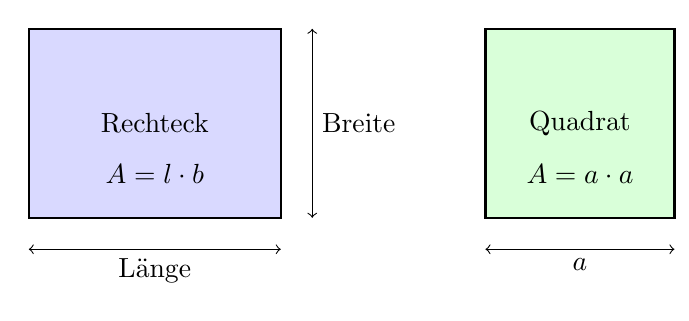
\begin{tikzpicture}[scale=0.8]
    % Rechteck
    \begin{scope}[xshift=0cm]
        \fill[blue!15] (0,0) rectangle (4,3);
        \draw[thick] (0,0) rectangle (4,3);
        \draw[<->] (0,-0.5) -- (4,-0.5) node[midway, below] {Länge};
        \draw[<->] (4.5,0) -- (4.5,3) node[midway, right] {Breite};
        \node at (2,1.5) {Rechteck};
        \node at (2,0.7) {$A = l \cdot b$};
    \end{scope}
    \hspace{1cm}
    % Quadrat
    \begin{scope}[xshift=6cm]
        \fill[green!15] (0,0) rectangle (3,3);
        \draw[thick] (0,0) rectangle (3,3);
        \draw[<->] (0,-0.5) -- (3,-0.5) node[midway, below] {$a$};
        \draw[<->] (3.5,0) -- (3.5,3) node[midway, right] {$a$};
        \node at (1.5,1.5) {Quadrat};
        \node at (1.5,0.7) {$A = a \cdot a$};
    \end{scope}
\end{tikzpicture}
\end{center}

\vspace{0.5em}

\subsection*{2. Berechne die Flächen der Rechtecke}

\begin{multicols}{2}
\begin{enumerate}[a)]
    \item Länge: 5 cm, Breite: 3 cm
    \item Länge: 7 cm, Breite: 4 cm
    \item Länge: 12 cm, Breite: 6 cm
    \item Länge: 4 m, Breite: 3 m
    \item Länge: 8 dm, Breite: 5 dm
    \item Länge: 10 mm, Breite: 5 mm
\end{enumerate}
\end{multicols}

\vspace{0.5em}

\subsection*{3. Berechne die Flächen der Quadrate}

\begin{multicols}{2}
\begin{enumerate}[a)]
    \item Seitenlänge: 4 cm
    \item Seitenlänge: 7 cm
    \item Seitenlänge: 10 cm
    \item Seitenlänge: 3 m
    \item Seitenlänge: 5 dm
    \item Seitenlänge: 20 mm
\end{enumerate}
\end{multicols}

\vspace{0.5em}

\subsection*{4. Zusammengesetzte Figuren}

Berechne den Flächeninhalt der schraffierten Flächen:

\begin{center}
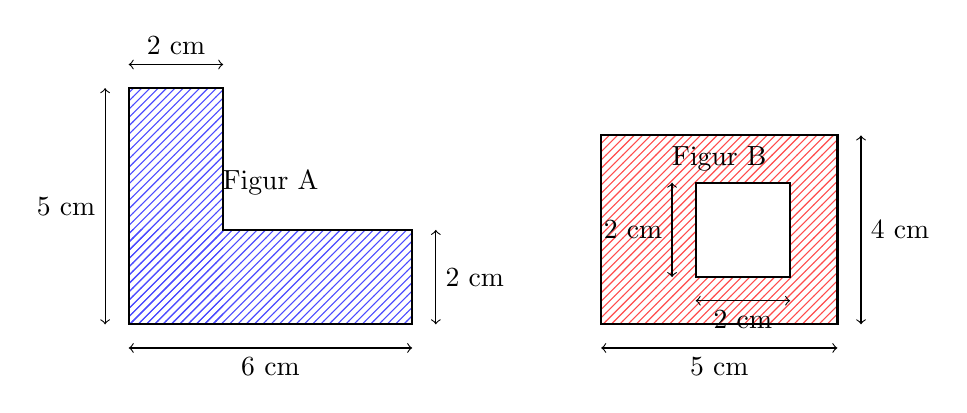
\begin{tikzpicture}[scale=0.6]
    % Figur 1: L-Form aus Rechtecken
    \begin{scope}[xshift=0cm]
        \fill[pattern=north east lines, pattern color=blue!70] (0,0) rectangle (6,2);
        \fill[pattern=north east lines, pattern color=blue!70] (0,0) rectangle (2,5);
        \draw[thick] (0,0) -- (6,0) -- (6,2) -- (2,2) -- (2,5) -- (0,5) -- cycle;
        
        % Maße
        \draw[<->] (0,-0.5) -- (6,-0.5) node[midway, below] {6 cm};
        \draw[<->] (6.5,0) -- (6.5,2) node[midway, right] {2 cm};
        \draw[<->] (-0.5,0) -- (-0.5,5) node[midway, left] {5 cm};
        \draw[<->] (0,5.5) -- (2,5.5) node[midway, above] {2 cm};
        
        \node at (3,3) {Figur A};
    \end{scope}
    
    % Figur 2: Zusammengesetztes Rechteck mit Aussparung
    \begin{scope}[xshift=10cm]
        \fill[pattern=north east lines, pattern color=red!70] (0,0) rectangle (5,4);
        \fill[white] (2,1) rectangle (4,3);
        \draw[thick] (0,0) rectangle (5,4);
        \draw[thick] (2,1) rectangle (4,3);
        
        % Maße
        \draw[<->] (0,-0.5) -- (5,-0.5) node[midway, below] {5 cm};
        \draw[<->] (5.5,0) -- (5.5,4) node[midway, right] {4 cm};
        \draw[<->] (2,0.5) -- (4,0.5) node[midway, below] {2 cm};
        \draw[<->] (1.5,1) -- (1.5,3) node[midway, left] {2 cm};
        
        \node at (2.5,3.5) {Figur B};
    \end{scope}
\end{tikzpicture}
\end{center}

\vspace{0.5em}

\subsection*{5. Einheiten umwandeln und Flächen berechnen}

Wandle die Längen in die angegebene Einheit um und berechne dann den Flächeninhalt:

\begin{enumerate}[a)]
    \item Ein Rechteck mit Länge 1 m und Breite 50 cm (in cm²)
    \item Ein Quadrat mit Seitenlänge 3 dm (in cm²)
    \item Ein Rechteck mit Länge 300 mm und Breite 2 dm (in cm²)
    \item Ein Quadrat mit Seitenlänge 0,5 m (in dm²)
    \item Ein Rechteck mit Länge 1 m und Breite 80 cm (in m²)
\end{enumerate}

\vspace{0.5em}

\subsection*{6. Praktische Aufgaben}

\begin{enumerate}[a)]
    \item Ein Klassenzimmer ist 8 m lang und 6 m breit. Wie groß ist die Fläche des Zimmers?
    
    \item Familie Müller will ihr Wohnzimmer renovieren. Der Raum ist rechteckig mit 5 m Länge und 4 m Breite. Der Quadratmeter Teppichboden kostet 19 €. Wie viel müssen sie für den neuen Teppich bezahlen?
    
    \item Ein Gärtner möchte ein rechteckiges Blumenbeet mit 3 m Länge und 2 m Breite anlegen. Er braucht pro Quadratmeter 8 Blumen. Wie viele Blumen muss er kaufen?
    
    \item Die Tafel im Klassenzimmer ist rechteckig mit einer Länge von 2 m und einer Höhe von 1,2 m. Wie groß ist die Fläche der Tafel?
\end{enumerate}

% \vspace{0.5em}

% \subsection*{7. Knobel-Aufgaben}

% \begin{center}
% \begin{tikzpicture}[scale=0.7]
%     % Schachbrett
%     \begin{scope}[xshift=0cm]
%         \foreach \i in {0,...,7} {
%             \foreach \j in {0,...,7} {
%                 \pgfmathparse{mod(\i+\j,2) ? "white" : "black"}
%                 \fill[\pgfmathresult] (\i,\j) rectangle +(1,1);
%             }
%         }
%         \draw[thick] (0,0) rectangle (8,8);
        
%         \node at (4,-1) {Figur C: Ein Schachbrett mit $8 \times 8$ Feldern};
%     \end{scope}
    
    % Tangram-ähnliche Figur
%     \begin{scope}[xshift=12cm]
%         \fill[blue!20] (0,0) -- (4,0) -- (4,4) -- (0,4) -- cycle;
%         \fill[red!20] (0,0) -- (2,2) -- (0,4) -- cycle;
%         \fill[green!20] (4,0) -- (2,2) -- (4,4) -- cycle;
%         \draw[thick] (0,0) -- (4,0) -- (4,4) -- (0,4) -- cycle;
%         \draw[thick] (0,0) -- (2,2) -- (4,0);
%         \draw[thick] (0,4) -- (2,2) -- (4,4);
        
%         % Maße
%         \draw[<->] (0,-0.5) -- (4,-0.5) node[midway, below] {4 cm};
%         \draw[<->] (4.5,0) -- (4.5,4) node[midway, right] {4 cm};
        
%         \node at (2,-1) {Figur D: Zusammengesetzte Figur};
%     \end{scope}
% \end{tikzpicture}
% \end{center}

% \begin{enumerate}[a)]
%     \item Wie viele schwarze Felder hat das Schachbrett (Figur C)?
%     \item Wie groß ist die Fläche eines einzelnen Feldes, wenn das Schachbrett eine Seitenlänge von 24 cm hat?
%     \item Berechne die Fläche jedes farbigen Teils in Figur D.
%     \item Die ganze Figur D hat eine Fläche von 16 cm². Beweise, dass alle Teilflächen zusammen auch 16 cm² ergeben.
% \end{enumerate}

\vspace{1em}

\textbf{Tipp}: Bei zusammengesetzten Figuren kannst du die Fläche in einfache Rechtecke und Quadrate aufteilen und diese einzeln berechnen!